\documentclass[11pt,a4paper]{article}

\usepackage[utf8]{inputenc}
\usepackage[T1]{fontenc}
\usepackage[spanish,es-nodecimaldot]{babel}
\usepackage{lmodern}
\usepackage{microtype}
\usepackage[a4paper,margin=2.5cm]{geometry}
\usepackage{graphicx}
\usepackage{booktabs}
\usepackage{tabularx}
\usepackage{longtable}
\usepackage{array}
\usepackage{float}
\usepackage{enumitem}
\usepackage{xcolor}
\usepackage{fancyhdr}
\usepackage{titlesec}
\usepackage[numbers]{natbib}
\usepackage[hidelinks]{hyperref}

\definecolor{spotifygreen}{HTML}{1DB954}
\definecolor{spotifydark}{HTML}{191414}
\definecolor{softgray}{HTML}{F2F4F5}
\graphicspath{{../../reports/figures/}}
\newcommand{\code}[1]{\texttt{\detokenize{#1}}}
\newcommand{\risk}[1]{\textbf{#1}}
\renewcommand{\arraystretch}{1.15}
\setlist{nosep,leftmargin=*}
\setlist[description]{style=nextline,leftmargin=0pt}
\setlength{\parskip}{0.45em}
\setlength{\parindent}{0pt}
\setlength{\headheight}{14pt}
\setlength{\emergencystretch}{3em}
\pagestyle{fancy}
\fancyhf{}
\lhead{Spotify Popularity Analysis}
\rhead{Informe técnico extendido}
\cfoot{\thepage}
\titleformat{\section}{\Large\bfseries\color{spotifydark}}{\thesection}{0.7em}{}
\titleformat{\subsection}{\large\bfseries\color{spotifydark}}{\thesubsection}{0.7em}{}

\title{\textbf{Spotify Popularity Analysis}\\[0.4em]
\large Informe técnico extendido y apoyo para defensa}
\author{Lucas Moncada \and Ignacio Silva \and César Rojas}
\date{11 de septiembre de 2026}

\begin{document}

\maketitle
\begin{center}
\fcolorbox{spotifygreen}{softgray}{\parbox{0.87\textwidth}{
Este documento complementa el README y los notebooks. Consolida evidencia, decisiones,
limitaciones y argumentos para defensa; no sustituye los artefactos ejecutables ni constituye
un modelo predictivo terminado.}}
\end{center}

\tableofcontents
\clearpage

\section{Resumen ejecutivo}

Este proyecto estudia qué características musicales y contextuales están asociadas con la
popularidad observada de canciones en Spotify. Su propósito es aportar evidencia para artistas,
sellos, marketing, curadores y gestión de catálogo, sin presentar las asociaciones como causas ni
como una receta de éxito. El trabajo sigue CRISP-DM y conserva trazabilidad mediante Git, notebooks
ejecutables, funciones en Python, pruebas automatizadas y documentación de progreso.

La fuente entregada por la asignatura contiene 114.000 filas y 21 columnas. No representa 114.000
canciones diferentes: solo existen 89.741 valores únicos de \code{track_id}; 16.641 IDs aparecen
más de una vez y generan 24.259 apariciones adicionales. Se detectaron tres celdas nulas, todas en
una fila que además posee duración cero, y una columna técnica \code{Unnamed: 0} que reproduce el
índice exportado. La distribución por género original contiene exactamente 1.000 filas para cada
una de 114 etiquetas, indicio de un diseño de muestra balanceado y no de la prevalencia real del
catálogo.

La preparación retiró la columna técnica y la única fila inválida. Después consolidó cada
\code{track_id}, verificando que sus atributos musicales y textuales fueran invariantes. Las
etiquetas de género se conservaron como una lista ordenada separada por barras verticales en
\code{track_genres}; cuando un ID presentaba diferentes valores históricos de popularidad, se usó
la mediana. El resultado contiene 89.740 canciones únicas, 20 columnas, cero nulos, cero IDs
duplicados y duración estrictamente positiva.

\begin{table}[H]
\centering
\caption{Comparación reproducible del dataset antes y después de la preparación.}
\label{tab:comparacion-resumen}
\resizebox{\textwidth}{!}{\begin{tabular}{lrrrrrr}
\toprule
 & Filas & Canciones unicas & Media & Mediana & Porcentaje igual a 0 & Porcentaje mayor o igual a 70 \\
dataset &  &  &  &  &  &  \\
\midrule
Original & 114000 & 89741 & 33.239 & 35.000 & 14.053 & 4.800 \\
Procesado & 89740 & 89740 & 33.198 & 33.000 & 10.468 & 3.480 \\
\bottomrule
\end{tabular}
}
\end{table}

El EDA procesado obtiene una popularidad media de 33,20, mediana de 33 y desviación estándar de
20,58. El 10,47\% de las canciones tiene popularidad cero y el 3,48\% alcanza 70 o más. Ningún
atributo acústico individual muestra una asociación fuerte con el objetivo. La mayor magnitud es
\code{instrumentalness} (Pearson $-0{,}128$; Spearman $-0{,}124$); \code{loudness} y
\code{danceability} presentan asociaciones positivas pequeñas. Entre predictores sí aparecen
redundancias relevantes: \code{energy} con \code{loudness} ($0{,}759$) y con
\code{acousticness} ($-0{,}733$).

Las canciones marcadas como explícitas tienen una media 4,03 puntos superior y una mediana cuatro
puntos superior, pero el tamaño de efecto estandarizado es pequeño ($d=0{,}196$). Esto distingue
una diferencia visible en una muestra grande de una diferencia práctica considerable. El ranking
por género es estable al exigir soportes mínimos de 100, 200 o 500 canciones, aunque esa estabilidad
no corrige el muestreo artificialmente balanceado ni convierte las diferencias en efectos causales.

Los riesgos principales son la falta de temporalidad, variables contextuales omitidas, posible
memorización de artistas, leakage mediante identificadores, alta cardinalidad y deriva del concepto
de popularidad. Éticamente, un modelo podría reforzar ventajas existentes, reducir diversidad o
automatizar promoción de forma injustificada. El dataset no contiene datos directos de oyentes, por
lo que el riesgo de privacidad individual es relativamente bajo; aumentaría si se integraran
perfiles, ubicaciones o historiales de escucha.

El proyecto está preparado para una etapa inicial de modelamiento de regresión. Se recomienda
construir una línea base, excluir \code{track_id}, codificar géneros como multi-hot, evaluar con
MAE, RMSE y $R^2$, y documentar desempeño por segmentos. El resultado debe utilizarse como apoyo a
decisión humana, no como criterio único de mérito artístico, inversión o promoción.

\section{Introducción}

Las plataformas musicales generan metadatos y descriptores de audio que permiten caracterizar
catálogos a una escala difícil de abordar manualmente. En este contexto, la inteligencia musical
puede ayudar a describir segmentos, detectar patrones y priorizar preguntas de negocio. Sin
embargo, la disponibilidad de atributos no implica que la popularidad pueda explicarse solo por la
estructura sonora: la exposición, la promoción, la recencia y el reconocimiento previo también
intervienen y no están observados en este dataset.

El proyecto analiza la relación entre atributos de canciones y \code{popularity}. Su alcance actual
incluye comprensión del problema, evaluación de la fuente, preparación, EDA y recomendaciones para
modelamiento. No incluye todavía un modelo entrenado ni una evaluación predictiva fuera de muestra.

Conviene distinguir tres conceptos:

\begin{itemize}
\item \textbf{Asociación:} dos variables cambian de forma relacionada en los datos observados. Pearson y
Spearman cuantifican formas específicas de asociación.
\item \textbf{Predicción:} un procedimiento estima valores para observaciones no usadas al ajustarlo. Requiere
particiones y métricas fuera de muestra.
\item \textbf{Causalidad:} un cambio deliberado en una variable produciría un cambio en otra. Exige un diseño
causal, supuestos o evidencia que este estudio observacional no proporciona.
\end{itemize}

Por tanto, frases como ``mayor sonoridad causa popularidad'' o ``la música explícita tiene éxito'' no
están respaldadas. El lenguaje correcto describe patrones de la muestra y formula hipótesis para
validaciones futuras.

\section{Problema de negocio}

Artistas y organizaciones musicales deben decidir qué lanzamientos priorizar, cómo organizar un
catálogo y dónde concentrar recursos promocionales sin conocer completamente el desempeño futuro.
La pregunta central es:

\begin{quote}
¿Qué características musicales y contextuales están asociadas con la popularidad de una canción y
cómo puede esta información apoyar decisiones de promoción y gestión de catálogo?
\end{quote}

Los principales interesados y usos prudentes son:

\begin{itemize}
\item \textbf{Artistas:} comprender cómo se ubica una obra dentro de perfiles descriptivos, sin
convertirlos en reglas creativas.
\item \textbf{Sellos:} complementar revisión experta al priorizar experimentos o análisis de catálogo.
\item \textbf{Marketing musical:} caracterizar segmentos y formular campañas que luego deben medirse.
\item \textbf{Gestión de catálogo:} detectar grupos que requieren análisis específico y mantener una
visión documentada de cobertura.
\item \textbf{Curadores:} apoyar exploración de diversidad, nunca reemplazar juicio editorial.
\end{itemize}

Las restricciones son sustanciales: no hay fecha de extracción ni de lanzamiento, inversión,
exposición en playlists, región o comportamiento de usuarios. La popularidad es histórica y
dinámica según Spotify \citep{spotify_track_api}. En consecuencia, el análisis puede orientar
preguntas y priorizaciones, pero no garantizar desempeño comercial ni valorar mérito artístico.

\section{Objetivos y KPIs}

\textbf{Objetivo general.} Analizar relaciones entre atributos musicales y contextuales y la
popularidad observada, dejando una base confiable y evidencia reproducible para evaluar modelos de
regresión.

\textbf{Objetivos específicos.}

\begin{enumerate}
\item comprender el problema, los interesados y las decisiones relevantes;
\item documentar procedencia, estructura y calidad de la fuente;
\item preparar una unidad de análisis de una canción por \code{track_id};
\item explorar distribuciones, relaciones, anomalías, redundancias y sesgos;
\item clasificar variables según utilidad y riesgo para modelamiento;
\item comunicar limitaciones éticas, de privacidad y de interpretación.
\end{enumerate}

\begin{table}[H]
\centering
\caption{Indicadores del proyecto y su función.}
\label{tab:kpis}
\begin{tabularx}{\textwidth}{p{2.6cm}p{4.2cm}X}
\toprule
Tipo & Indicador & Interpretación y uso \\
\midrule
Negocio & Media y mediana de popularidad & Describen el centro del catálogo observado; no son
metas de predicción por sí mismas. \\
Negocio & Proporción con popularidad $\geq 70$ & Segmento operativo de alta popularidad; el umbral
no es una categoría oficial de Spotify. \\
Negocio & Popularidad por género & Compara segmentos con soporte; no estima prevalencia real ni
efecto causal. \\
Calidad & Completitud & Controla celdas disponibles y evita imputaciones injustificadas. \\
Calidad & Duplicidad de \code{track_id} & Verifica unidad de análisis y previene fuga entre
entrenamiento y prueba. \\
Modelo & MAE & Error absoluto promedio en puntos de popularidad, interpretable en la escala original. \\
Modelo & RMSE & Penaliza más los errores grandes y complementa MAE. \\
Modelo & $R^2$ & Proporción de variabilidad explicada respecto de una línea base; no mide causalidad. \\
\bottomrule
\end{tabularx}
\end{table}

Los KPIs de negocio describen utilidad potencial; las estadísticas descriptivas caracterizan la
muestra; y las métricas técnicas solo serán válidas al evaluarse fuera de muestra.

\section{Fuente de datos}

El archivo operativo es \code{data/raw/Spotify_Tracks_Dataset.csv}, proporcionado por la asignatura
y preservado sin modificaciones. Su estructura coincide con el conjunto publicado por Maharshi
Pandya en Kaggle \citep{pandya_dataset}. Esta coincidencia sustenta la descripción, pero la copia
local y su trazabilidad son la fuente efectiva del análisis.

El CSV original tiene 114.000 filas y 21 columnas. Incluye identificadores, artista, álbum, nombre
de pista, género, contenido explícito, duración y atributos acústicos. La variable objetivo
\code{popularity} está en escala 0--100. La documentación de Spotify la relaciona principalmente
con reproducciones y recencia, y el campo aparece actualmente como obsoleto en la API
\citep{spotify_track_api}. Se interpreta, por ello, como fotografía histórica y no como medición en
tiempo real.

La integridad de la copia raw se controla mediante SHA-256:

\begin{verbatim}
b202fa49909b2d5cef71a04b1d21243cfeb36414535f2ca9272aa646721177bd
\end{verbatim}

El diccionario completo está en \code{docs/data_dictionary.md}. En síntesis, los roles son:

\begin{table}[H]
\centering
\caption{Grupos de variables de la fuente.}
\label{tab:grupos-variables}
\begin{tabularx}{\textwidth}{p{3cm}X p{3.2cm}}
\toprule
Grupo & Variables representativas & Rol \\
\midrule
Identificación & \code{track_id} & Trazabilidad; no predictor \\
Contexto & \code{artists}, \code{album_name}, \code{track_name}, género & Segmentación y posible
alta cardinalidad \\
Audio & \code{danceability}, \code{energy}, \code{loudness}, \code{acousticness}, entre otras &
Predictores candidatos \\
Estructura musical & \code{key}, \code{mode}, \code{tempo}, \code{time_signature} & Predictores
categóricos o continuos según significado \\
Objetivo & \code{popularity} & Variable de respuesta histórica \\
Técnica & \code{Unnamed: 0} & Índice exportado, retirado \\
\bottomrule
\end{tabularx}
\end{table}

No se documenta la fecha exacta de extracción, la cobertura regional ni las condiciones completas
de muestreo. Esas ausencias limitan actualización, generalización temporal y representatividad.

\section{Metodología CRISP-DM}

CRISP-DM organiza el trabajo en seis fases iterativas \citep{crispdm}. Un hallazgo de calidad,
modelamiento o evaluación puede obligar a revisar una fase anterior; el flujo no es estrictamente
lineal.

\begin{table}[H]
\centering
\caption{Estado de CRISP-DM en el proyecto.}
\label{tab:crispdm}
\begin{tabularx}{\textwidth}{p{3.2cm}X p{3cm}}
\toprule
Fase & Aplicación & Estado \\
\midrule
Business Understanding & Problema, interesados, objetivos, KPIs y restricciones & Completada
inicialmente \\
Data Understanding & Fuente, diccionario, calidad inicial y distribuciones & Completada inicialmente \\
Data Preparation & Índice, fila inválida, consolidación de IDs y géneros múltiples & Completada
inicialmente \\
Modeling & Líneas base y regresiones justificadas & Pendiente \\
Evaluation & MAE, RMSE, $R^2$, utilidad, errores por grupos y robustez temporal & Pendiente \\
Deployment & Repositorio reproducible, informe y presentación & En construcción \\
\bottomrule
\end{tabularx}
\end{table}

La separación entre notebooks refleja responsabilidades: \code{01_data_understanding.ipynb}
documenta negocio y diagnóstico; \code{02_data_preparation.ipynb} transforma la fuente;
\code{03_exploratory_analysis.ipynb} estudia canciones únicas. La lógica común se implementa en
\code{src/spotify_popularity/} y se verifica en \code{tests/}.

\section{Comprensión inicial de los datos}

La inspección original confirmó 114.000 filas, 21 columnas, cero filas exactamente duplicadas y
89.741 IDs únicos. Hay 16.641 IDs repetidos que abarcan 40.900 filas; equivalen a 24.259
apariciones adicionales. En consecuencia, una fila representa una asignación pista--género y no
necesariamente una canción nueva.

Las tres celdas nulas corresponden a artista, álbum y nombre de una única fila. Esa misma fila tiene
duración cero. El bajo porcentaje de nulos no basta para concluir alta calidad: duplicidad
semántica, unidad de análisis y consistencia son más relevantes en este caso.

\begin{figure}[H]
\centering
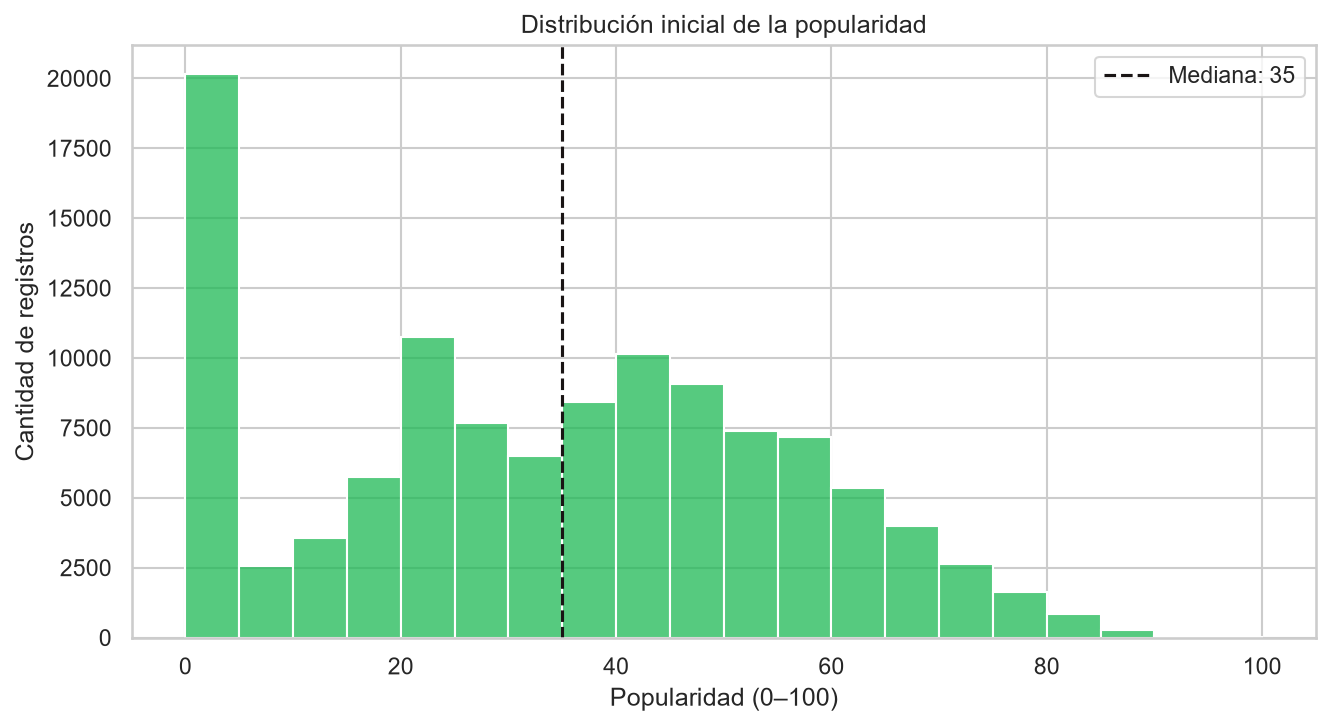
\includegraphics[width=0.82\textwidth]{01_popularity_distribution.png}
\caption{Distribución inicial de popularidad sobre 114.000 asignaciones pista--género. La media es
33,24 y la mediana 35; el gráfico todavía pondera varias veces canciones multigénero.}
\label{fig:popularidad-inicial}
\end{figure}

La Figura~\ref{fig:popularidad-inicial} permite diagnosticar concentración baja-media, pero no debe
interpretarse aún como distribución por canción única. El 14,05\% de las filas vale cero y el
4,80\% alcanza 70 o más.

\begin{figure}[H]
\centering
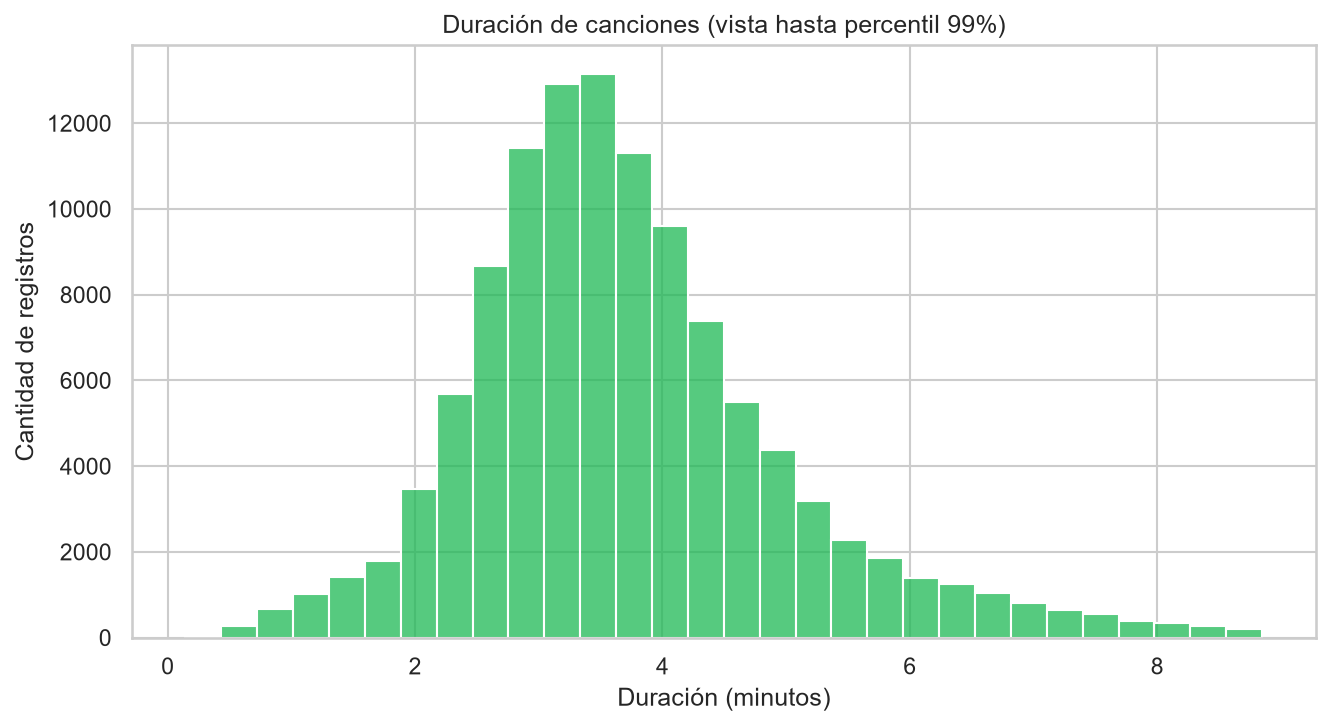
\includegraphics[width=0.82\textwidth]{02_duration_distribution.png}
\caption{Duración original limitada al percentil 99 para preservar legibilidad. El máximo no se
elimina y alcanza aproximadamente 87,29 minutos.}
\label{fig:duracion-inicial}
\end{figure}

La Figura~\ref{fig:duracion-inicial} separa visualización de decisión: recortar el eje no elimina
observaciones. La mediana original es 3,55 minutos y el percentil 99 es 8,85; la fila con duración
cero requiere tratamiento por combinar múltiples problemas de calidad.

\begin{figure}[H]
\centering
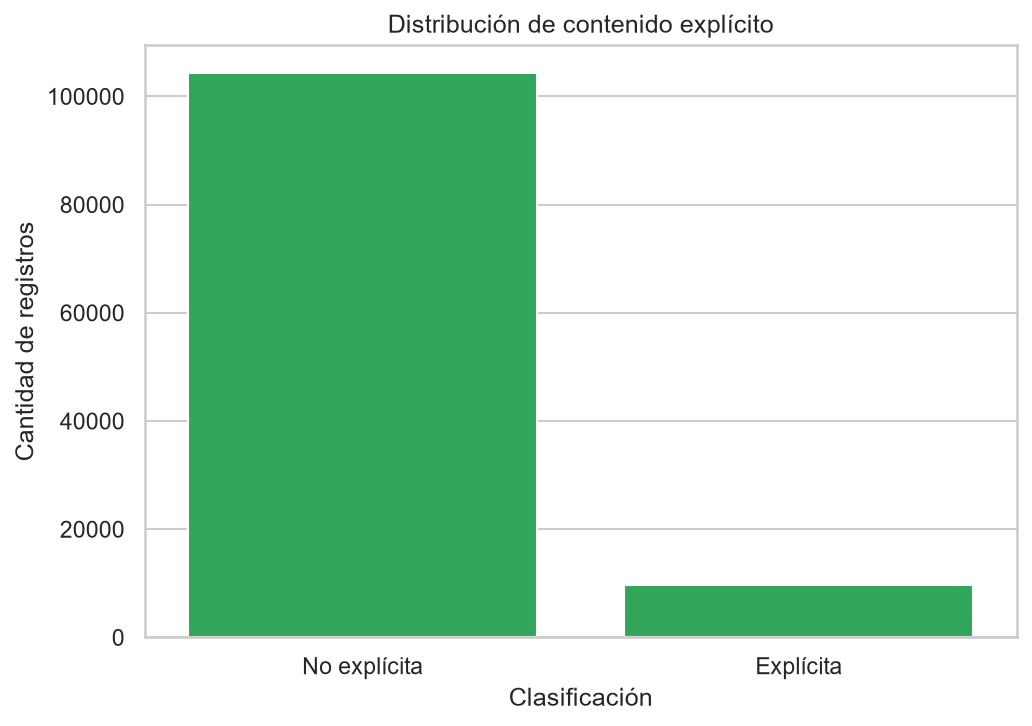
\includegraphics[width=0.72\textwidth]{03_explicit_distribution.png}
\caption{Conteo inicial de contenido explícito. Solo 8,55\% de las filas está marcado como
explícito; \code{False} no debe interpretarse más allá de la definición disponible.}
\label{fig:explicit-inicial}
\end{figure}

\begin{figure}[H]
\centering
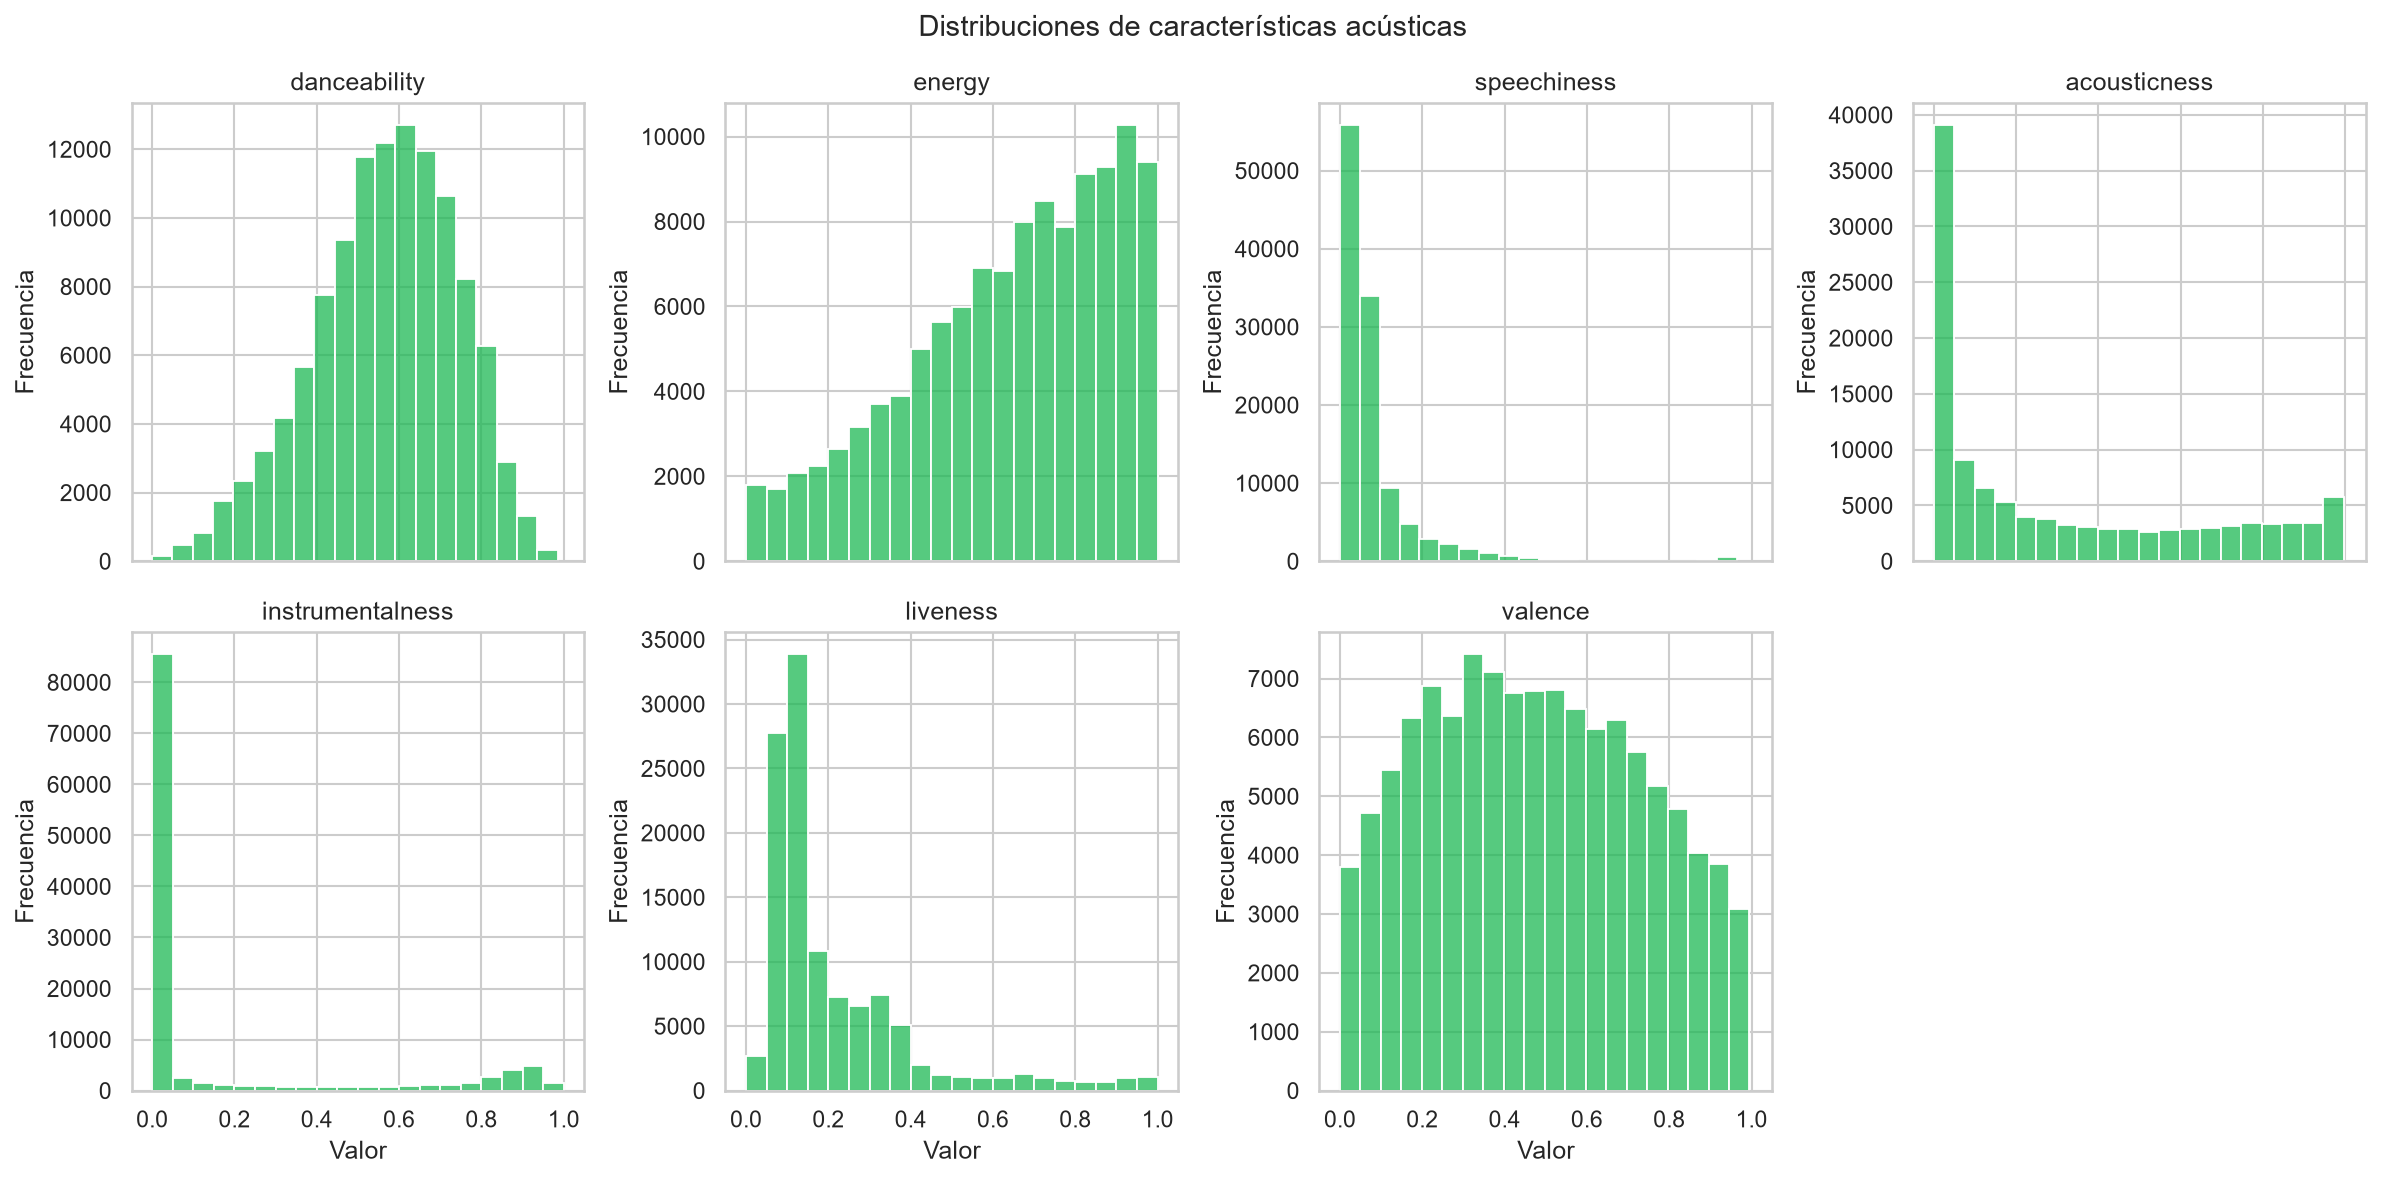
\includegraphics[width=\textwidth]{04_audio_feature_distributions.png}
\caption{Distribuciones iniciales de atributos acústicos. \code{speechiness},
\code{instrumentalness} y \code{liveness} concentran masa cerca de cero.}
\label{fig:audio-inicial}
\end{figure}

La Figura~\ref{fig:audio-inicial} anticipa asimetría y acumulaciones válidas en variables acotadas;
por ello media, IQR y gráficos deben interpretarse con sus formas distributivas. Finalmente, las
114 etiquetas de género tienen exactamente 1.000 filas cada una: esto facilita comparaciones con
soporte, pero es evidencia de balance artificial y no de prevalencia real.

\section{Calidad y preparación de datos}

La preparación se ejecuta desde la fuente inmutable mediante
\path{scripts/build_processed_dataset.py}. La implementación en
\path{src/spotify_popularity/data/preparation.py} valida esquema, detecta filas inválidas, comprueba
atributos invariantes y consolida IDs.

\begin{table}[H]
\centering
\caption{Problemas, decisiones y riesgos residuales de preparación.}
\label{tab:decisiones-preparacion}
\small
\begin{tabularx}{\textwidth}{p{2.5cm}p{3.1cm}p{2.7cm}X p{2.7cm}}
\toprule
Problema & Evidencia & Decisión & Justificación & Riesgo residual \\
\midrule
Índice exportado & Secuencia \code{Unnamed: 0} & Retirar del derivado & No describe una canción y podría introducir orden artificial & Ninguno relevante \\
Fila inválida & Tres textos nulos y duración cero & Excluir una fila & No hay evidencia para imputar identidad ni duración & Posible pérdida mínima de cobertura \\
IDs repetidos & 16.641 IDs; 24.259 apariciones extra & Consolidar por \code{track_id} & Evita doble conteo y fuga entre particiones & La popularidad histórica se resume \\
Géneros múltiples & Una pista puede aparecer en varias etiquetas & Unir etiquetas únicas con \code{|} & Conserva información sin duplicar canciones & Requiere encoding multietiqueta \\
Popularidad variable & 720 IDs repetidos difieren en el objetivo & Usar mediana & Es determinista y robusta sin privilegiar el orden del archivo & No representa actualidad ni trayectoria \\
\bottomrule
\end{tabularx}
\end{table}

Elegir la primera fila habría vinculado el resultado al orden del CSV; promediar sería más sensible
a discrepancias extremas; eliminar todos los IDs repetidos descartaría información válida. La
mediana y la preservación de etiquetas equilibran trazabilidad, robustez y retención de datos. El
código se detiene si atributos declarados invariantes entran en conflicto, evitando consolidaciones
silenciosas.

El contrato posterior confirma 89.740 filas y 20 columnas, 89.740 IDs únicos, cero celdas nulas,
cero duraciones no positivas y géneros no vacíos. Estas comprobaciones validan la entrada al EDA,
pero no eliminan sesgos de origen ni garantizan representatividad.

\subsection{Comparación antes y después}

\begin{table}[H]
\centering
\caption{Impacto cuantitativo de consolidar \code{track_id}. Tabla generada por
\code{scripts/build_latex_tables.py}.}
\label{tab:antes-despues}
\resizebox{\textwidth}{!}{\begin{tabular}{lrrrrrr}
\toprule
 & Filas & Canciones unicas & Media & Mediana & Porcentaje igual a 0 & Porcentaje mayor o igual a 70 \\
dataset &  &  &  &  &  &  \\
\midrule
Original & 114000 & 89741 & 33.239 & 35.000 & 14.053 & 4.800 \\
Procesado & 89740 & 89740 & 33.198 & 33.000 & 10.468 & 3.480 \\
\bottomrule
\end{tabular}
}
\end{table}

La tabla~\ref{tab:antes-despues} muestra que las canciones únicas pasan de 89.741 a 89.740 por la
exclusión de la fila inválida, mientras las filas caen 21,28\%. La media apenas cambia (33,24 a
33,20), pero la mediana baja de 35 a 33, la masa en cero de 14,05\% a 10,47\% y el segmento de 70 o
más de 4,80\% a 3,48\%. Esto demuestra que la duplicación por género modificaba la ponderación de
la distribución: incluso si la media permanece cercana, otras características relevantes cambian.

\section{Análisis exploratorio profundo}

El EDA se realiza sobre una fila por canción. Este cambio hace que cada estadística responda a la
unidad de negocio elegida y no a la cantidad de etiquetas de género asociadas.

\subsection{Distribución procesada de popularidad}

La media es 33,198, la mediana 33, la desviación estándar 20,578, los percentiles 25 y 75 son 19 y
49, y el percentil 95 es 67. El rango completo 0--100 es compatible con la escala documentada.

\begin{figure}[H]
\centering
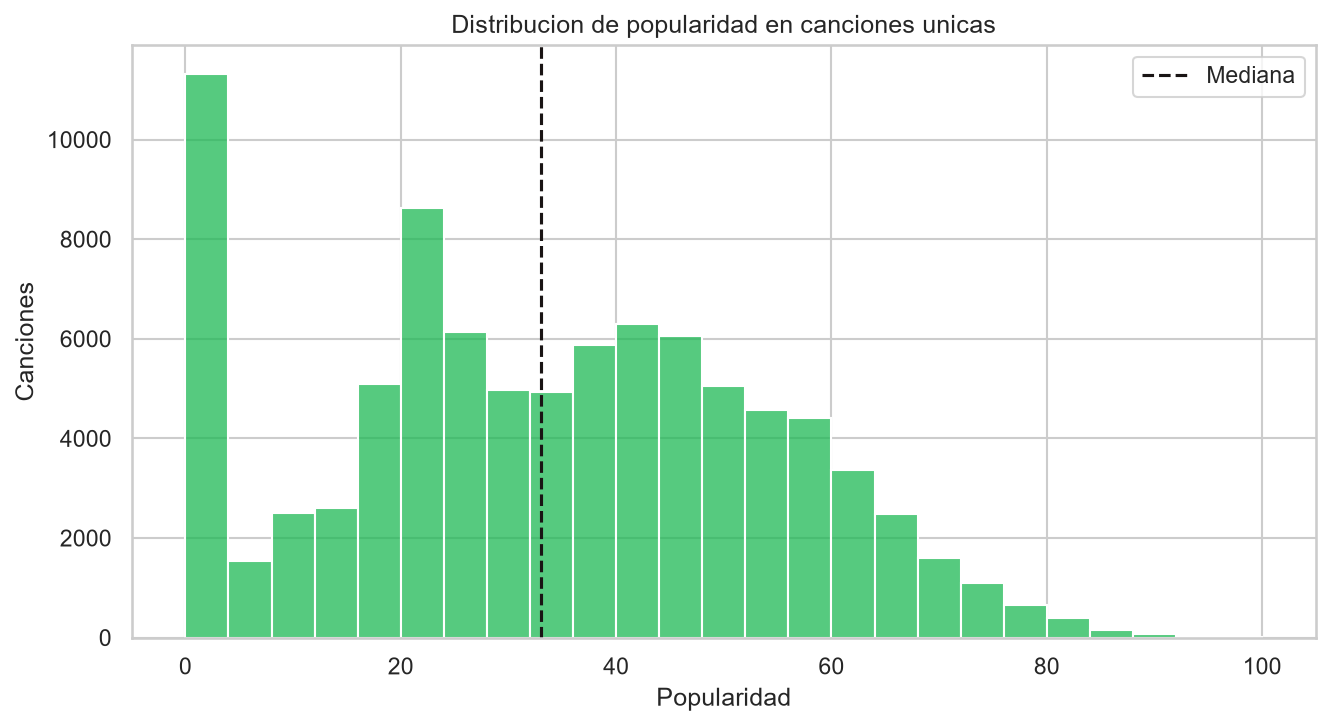
\includegraphics[width=0.84\textwidth]{05_processed_popularity_distribution.png}
\caption{Popularidad de 89.740 canciones únicas. La concentración baja-media y la masa en cero son
relevantes para líneas base y evaluación por segmentos.}
\label{fig:popularidad-procesada}
\end{figure}

La Figura~\ref{fig:popularidad-procesada} importa porque define la dificultad del objetivo y
advierte que una métrica global puede ocultar errores distintos en canciones de baja y alta
popularidad. Los valores 0 y 100 no son errores solo por estar en los extremos. La limitación es que
la distribución describe una captura histórica sin fecha de referencia.

\subsection{Pearson y Spearman}

Pearson resume covariación lineal; Spearman calcula asociación monotónica sobre rangos y es menos
dependiente de una relación lineal exacta. La comparación evita concluir a partir de una sola forma.

\begin{table}[H]
\centering
\caption{Correlaciones con \code{popularity}, ordenadas por magnitud de Spearman.}
\label{tab:correlaciones-target}
\begin{tabular}{lrr}
\toprule
 & Pearson & Spearman \\
variable &  &  \\
\midrule
instrumentalness & -0.127 & -0.124 \\
loudness & 0.072 & 0.067 \\
speechiness & -0.047 & -0.067 \\
danceability & 0.064 & 0.055 \\
energy & 0.014 & -0.016 \\
duration\_ms & -0.023 & 0.013 \\
liveness & -0.014 & -0.012 \\
valence & -0.012 & -0.011 \\
acousticness & -0.039 & 0.010 \\
tempo & 0.007 & 0.008 \\
\bottomrule
\end{tabular}

\end{table}

Todas las magnitudes son pequeñas. \code{instrumentalness} es la señal negativa más visible;
\code{loudness} y \code{danceability} son positivas débiles. Diferencias de signo entre métodos,
como en \code{acousticness} y \code{duration_ms}, sugieren formas no lineales, empates o patrones
segmentados. La implicancia es evaluar modelos multivariables sin esperar gran poder explicativo de
un atributo aislado. La limitación central es que correlación no controla confusores ni implica
causalidad.

\subsection{Matriz de correlación y redundancia}

\begin{figure}[H]
\centering
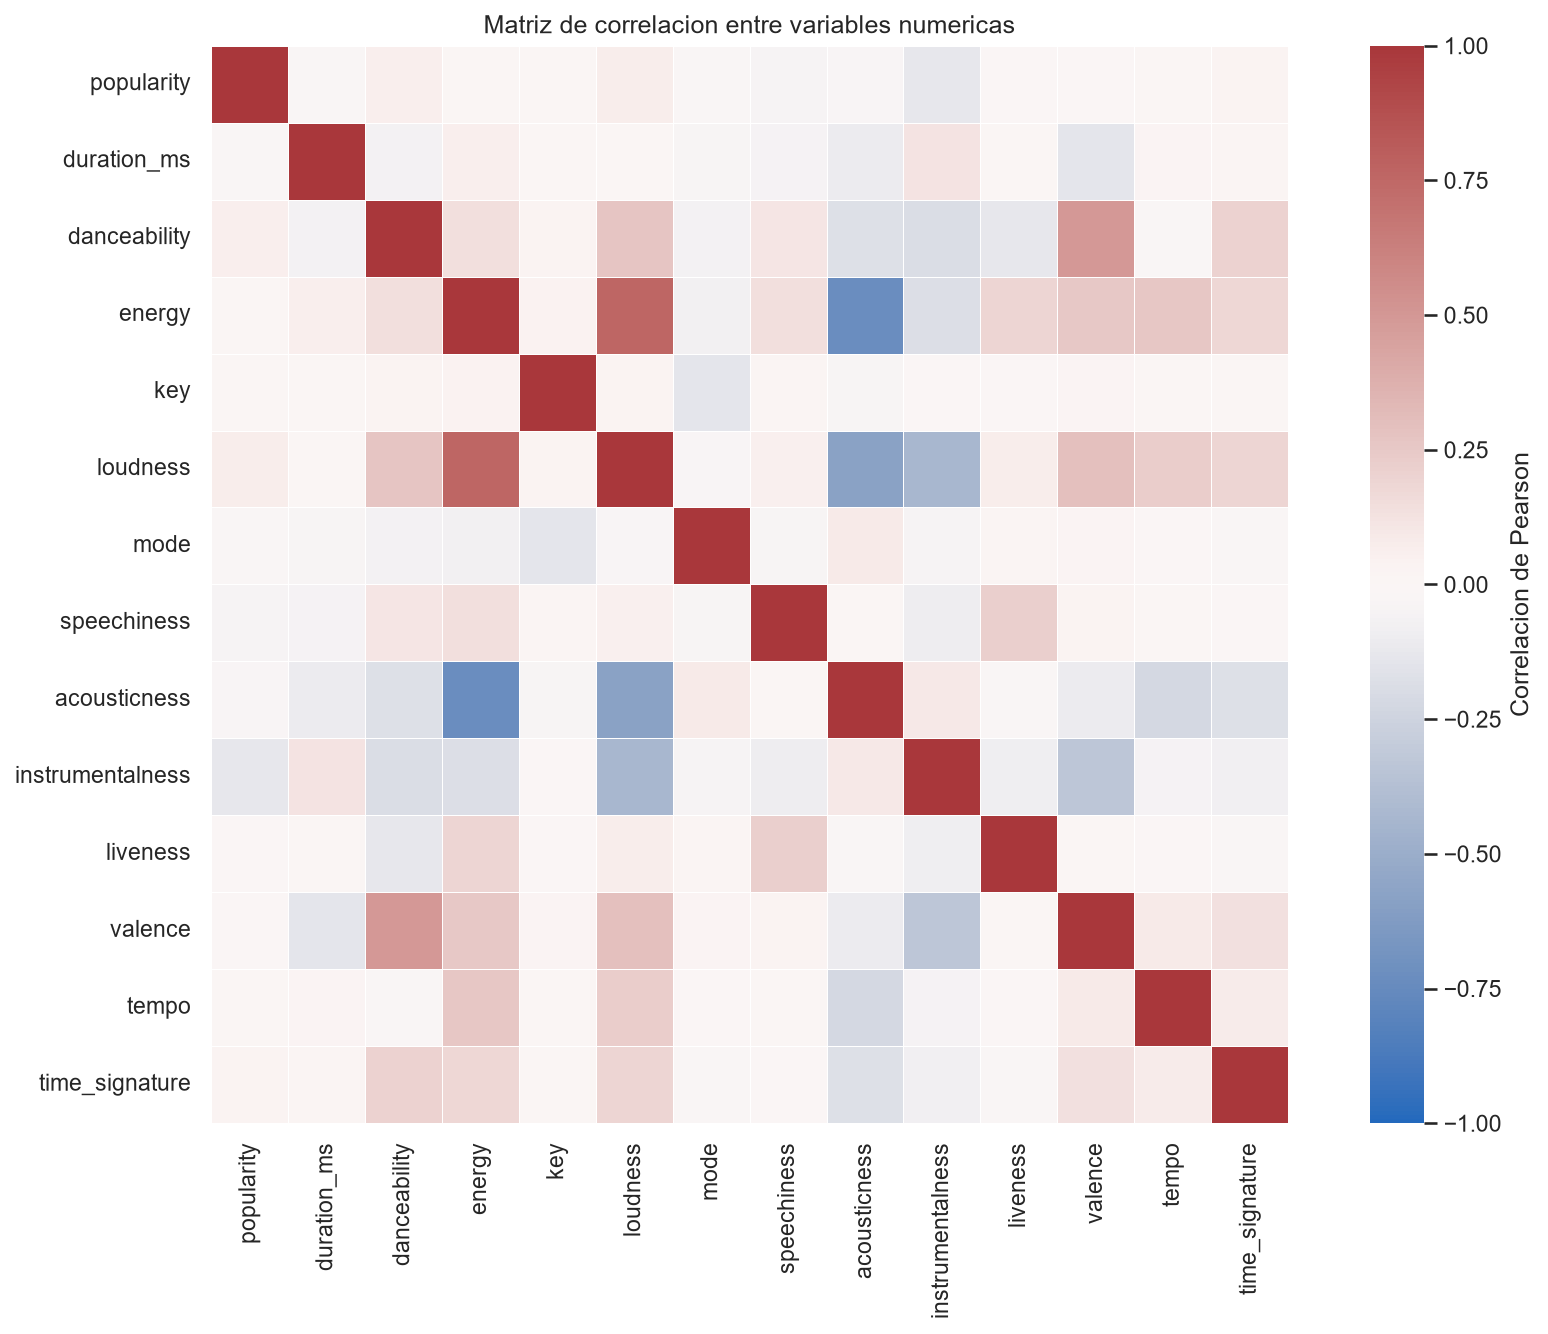
\includegraphics[width=0.91\textwidth]{06_numeric_correlation_heatmap.png}
\caption{Matriz de Pearson para variables numéricas. Las celdas más intensas aparecen entre
predictores de audio, no con el objetivo.}
\label{fig:matriz-correlacion}
\end{figure}

La Figura~\ref{fig:matriz-correlacion} permite detectar redundancia: \code{energy}--\code{loudness}
alcanza 0,759; \code{energy}--\code{acousticness}, $-0{,}733$; y
\code{loudness}--\code{acousticness}, $-0{,}583$. Para regresión lineal, coeficientes asociados
pueden volverse inestables y difíciles de interpretar. Esto no obliga a retirar variables: permite
planificar regularización y diagnóstico. La matriz solo refleja relaciones pares y lineales.

\subsection{Relaciones bivariadas por cuantiles}

Un scatterplot con casi 90 mil puntos produciría sobreposición. Se dividen valores en cuantiles y se
representa la mediana de popularidad de cada intervalo, manteniendo todos los datos en el cálculo.

\begin{figure}[H]
\centering
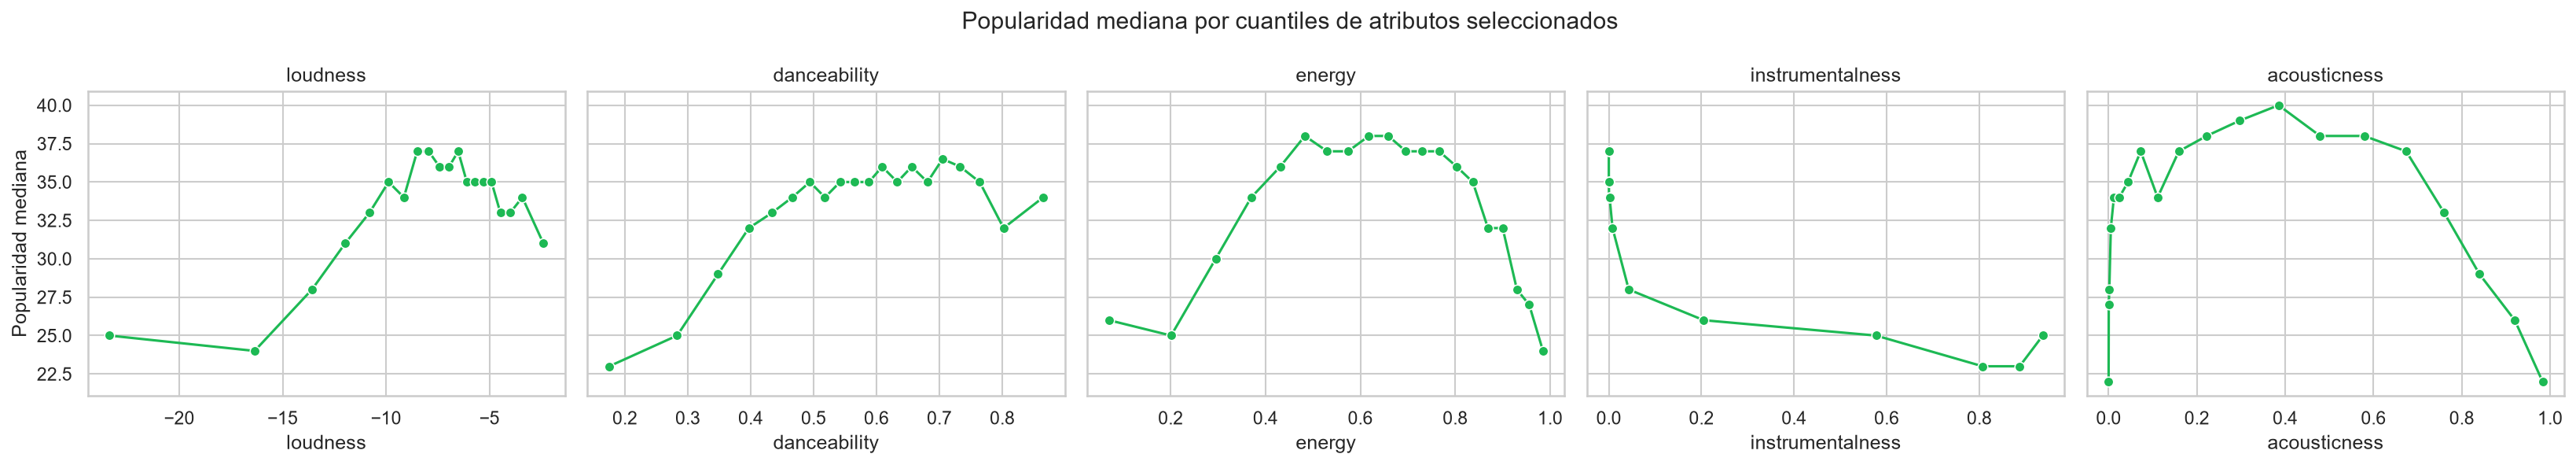
\includegraphics[width=\textwidth]{07_binned_feature_popularity.png}
\caption{Popularidad mediana por cuantiles de cinco atributos. Las curvas permiten observar forma y
no solo un coeficiente global.}
\label{fig:cuantiles-popularidad}
\end{figure}

La Figura~\ref{fig:cuantiles-popularidad} muestra caída más consistente con
\code{instrumentalness}; \code{loudness} y \code{danceability} crecen en parte del rango, pero no de
forma ilimitada. \code{energy} y \code{acousticness} exhiben curvatura. Esto respalda términos no
lineales o modelos flexibles como hipótesis de modelamiento, no reglas creativas. Los cuantiles
resumen heterogeneidad y pueden ocultar subgrupos por género o época.

\subsection{Contenido explícito y tamaño de efecto}

\begin{figure}[H]
\centering
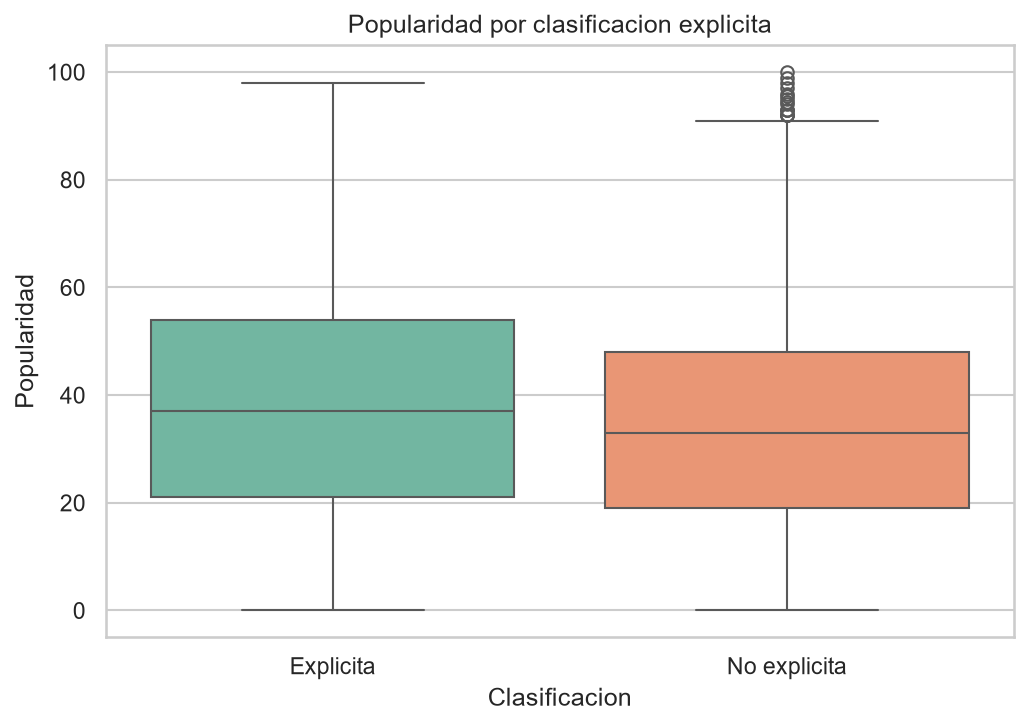
\includegraphics[width=0.72\textwidth]{08_explicit_popularity_boxplot.png}
\caption{Distribución de popularidad por clasificación explícita. El solapamiento entre grupos es
amplio pese a diferencias en los centros.}
\label{fig:explicit-popularidad}
\end{figure}

El grupo no explícito contiene 82.036 canciones y el explícito 7.704. Sus medias son 32,852 y
36,884; las medianas, 33 y 37. Para medir relevancia práctica se calculó $d$ de Cohen con desviación
estándar combinada \citep{cohen1988}.

\begin{table}[H]
\centering
\caption{Diferencias y tamaño de efecto de \code{explicit}.}
\label{tab:explicit-efecto}
\begin{tabular}{lr}
\toprule
 & Valor \\
\midrule
Canciones no explicitas & 82036.000 \\
Canciones explicitas & 7704.000 \\
Diferencia de medias & 4.032 \\
Diferencia de medianas & 4.000 \\
d de Cohen & 0.196 \\
\bottomrule
\end{tabular}

\end{table}

La diferencia de 4,03 puntos puede resultar estadísticamente detectable con una muestra grande,
pero $d=0{,}196$ indica separación estandarizada pequeña. La Figura~\ref{fig:explicit-popularidad}
confirma fuerte solapamiento. La asociación puede depender de género, público, recencia y
promoción; no prueba que hacer una canción explícita aumente popularidad.

\subsection{Géneros multietiqueta y sensibilidad}

Cada valor de \code{track_genres} se divide por \code{|}. Una canción puede participar en varias
etiquetas: las filas expandidas no constituyen canciones adicionales. El resumen cuenta IDs únicos
por etiqueta y exige soporte para evitar líderes de muestras mínimas.

\begin{figure}[H]
\centering
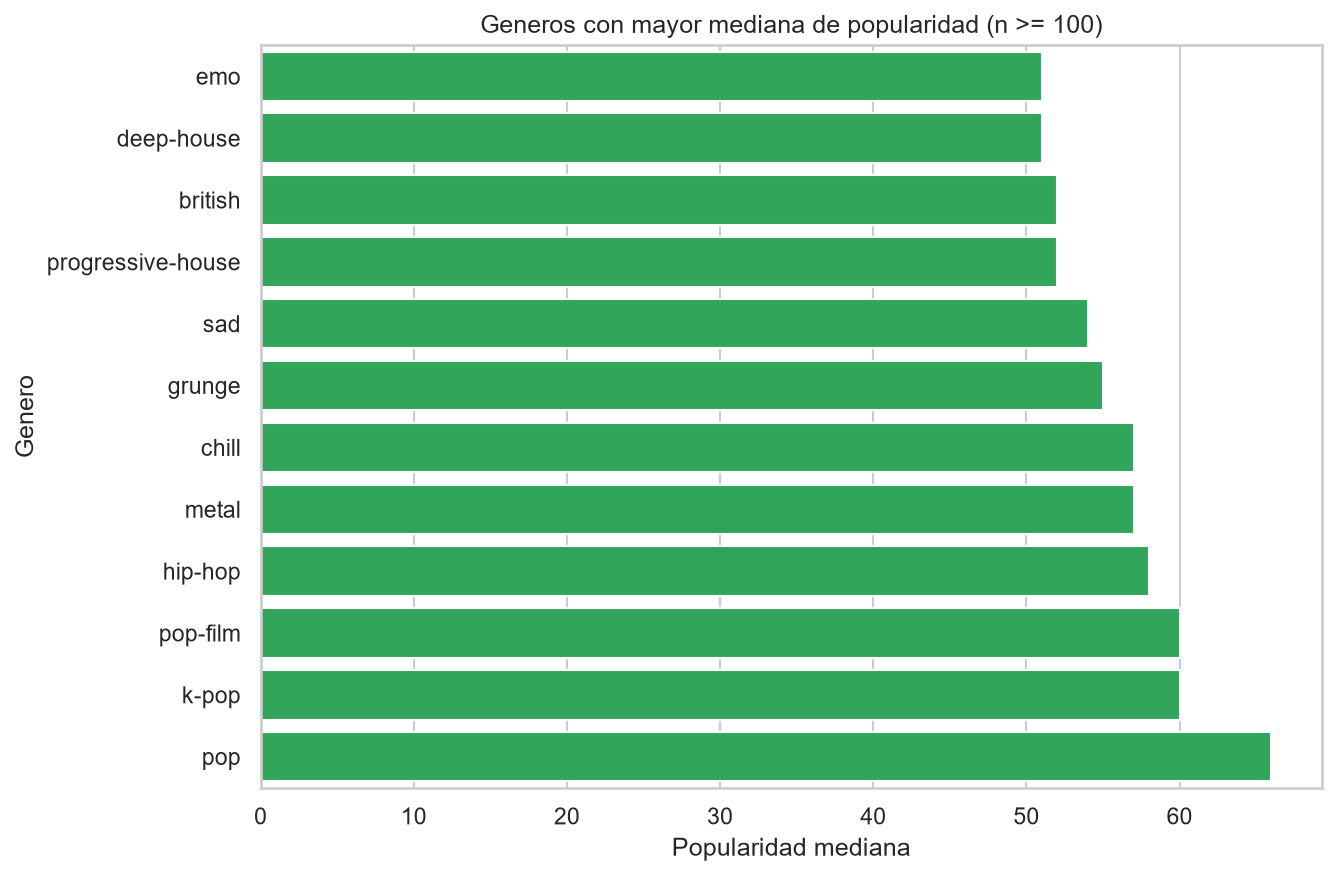
\includegraphics[width=0.82\textwidth]{09_genre_popularity_summary.png}
\caption{Géneros con mayor mediana de popularidad entre etiquetas con al menos 100 canciones.}
\label{fig:generos-popularidad}
\end{figure}

\begin{table}[H]
\centering
\caption{Sensibilidad del líder por mediana a distintos soportes mínimos.}
\label{tab:sensibilidad-generos}
\begin{tabular}{lrlr}
\toprule
 & Generos incluidos & Genero lider & Mediana lider \\
Soporte minimo &  &  &  \\
\midrule
100 & 114 & pop & 66.000 \\
200 & 114 & pop & 66.000 \\
500 & 114 & pop & 66.000 \\
\bottomrule
\end{tabular}

\end{table}

Los 114 géneros superan 100, 200 y 500 canciones, y \code{pop} mantiene mediana 66. Esto demuestra
estabilidad frente a esos umbrales en esta muestra, no superioridad universal. La Figura
\ref{fig:generos-popularidad} sirve para segmentar el dataset; su limitación es el balance artificial
del origen y la superposición de canciones entre etiquetas.

\subsection{Valores extremos}

El criterio IQR marca observaciones fuera de $[Q_1-1{,}5IQR, Q_3+1{,}5IQR]$. Es una regla de
identificación, no una prueba de error.

\begin{table}[H]
\centering
\caption{Rangos y recuentos fuera de IQR.}
\label{tab:extremos}
\resizebox{0.94\textwidth}{!}{\begin{tabular}{lrrrrr}
\toprule
 & Minimo & P1 & P99 & Maximo & Fuera de IQR \\
variable &  &  &  &  &  \\
\midrule
duration\_ms & 8586.000 & 61871.850 & 546010.980 & 5237295.000 & 4225 \\
tempo & 0.000 & 65.165 & 193.652 & 243.372 & 514 \\
loudness & -49.531 & -28.542 & -1.628 & 4.532 & 5026 \\
speechiness & 0.000 & 0.025 & 0.619 & 0.965 & 10644 \\
instrumentalness & 0.000 & 0.000 & 0.958 & 1.000 & 19613 \\
liveness & 0.000 & 0.041 & 0.950 & 1.000 & 6981 \\
\bottomrule
\end{tabular}
}
\end{table}

\begin{figure}[H]
\centering
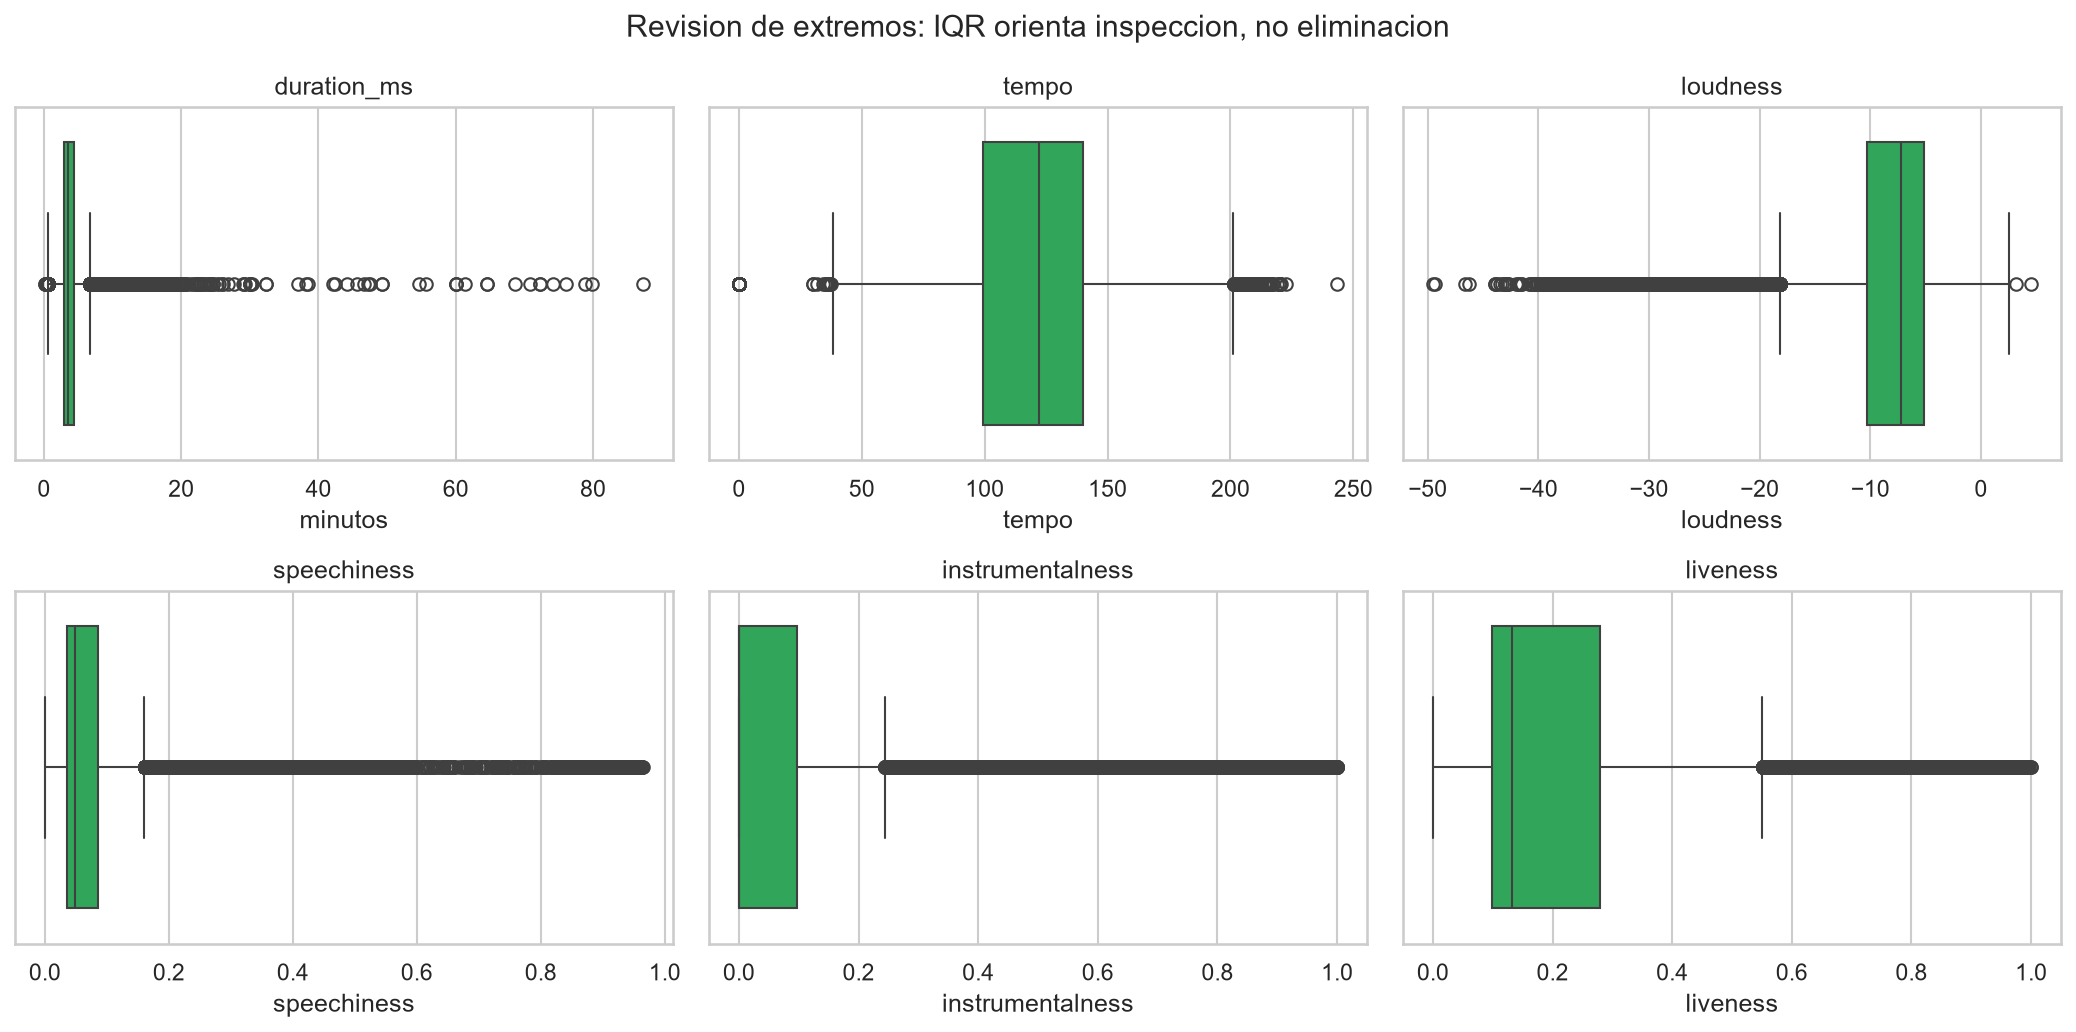
\includegraphics[width=0.93\textwidth]{10_outlier_review.png}
\caption{Revisión de extremos. Las colas largas y acumulaciones en cero requieren interpretación por
variable, no eliminación automática.}
\label{fig:revision-extremos}
\end{figure}

\code{duration_ms} alcanza 5.237.295 ms (87,29 minutos); puede representar contenido largo válido.
\code{tempo} incluye cero y merece validación puntual, pero no se infiere que sea inválido sin
metadatos adicionales. \code{loudness} llega a $-49{,}531$ y 4,532 dB. En
\code{speechiness}, \code{instrumentalness} y \code{liveness}, una gran cantidad fuera de IQR es
compatible con distribuciones asimétricas acotadas 0--1. La implicancia es probar transformaciones o
escaladores robustos y analizar sensibilidad; eliminar puntos podría borrar géneros completos o
casos legítimos.

\section{Análisis de variables y utilidad para modelamiento}

La tabla siguiente integra descripción estadística, relación observada y decisión técnica. Una
correlación débil no implica inutilidad multivariable: interacciones y relaciones no lineales pueden
aportar información, pero deben comprobarse fuera de muestra.

\small
\begin{longtable}{p{3.2cm}p{3.4cm}p{3.2cm}p{4.2cm}}
\caption{Síntesis de variables para la siguiente etapa.}\label{tab:analisis-variables}\\
\toprule
Variable & Descripción estadística & Relación con popularidad & Utilidad o riesgo \\
\midrule
\endfirsthead
\toprule
Variable & Descripción estadística & Relación con popularidad & Utilidad o riesgo \\
\midrule
\endhead
\code{danceability} & Continua 0--1, distribución amplia & Pearson 0,064; Spearman 0,055; curva por cuantiles & Candidata; permitir no linealidad \\
\code{energy} & Continua 0--1 & Asociación casi nula con target & Candidata, pero redundante con sonoridad y acousticness \\
\code{loudness} & dB con cola negativa & Pearson 0,072; Spearman 0,067 & Candidata; escalar y revisar extremos \\
\code{speechiness} & Masa cerca de cero y cola alta & Pearson -0,047; Spearman -0,067 & Candidata; posible transformación y segmentación \\
\code{acousticness} & Continua 0--1, relación no lineal & Pearson -0,039; Spearman 0,010 & Candidata con cautela por redundancia \\
\code{instrumentalness} & Acumulación en cero y valores altos & Mayor asociación: -0,128/-0,124 & Candidata; no convertir asociación en regla \\
\code{liveness} & Asimétrica y acotada & Cerca de cero & Mantener para prueba multivariable \\
\code{valence} & Distribución amplia 0--1 & Cerca de cero & Candidata; relacionada con danceability \\
\code{tempo} & Continua; incluye cero y máximo 243,372 & Cerca de cero & Validar extremos y escalar \\
\code{duration_ms} & Cola larga; máximo 87,29 minutos & Pearson -0,023; Spearman 0,013 & Evaluar \code{log1p} y escala robusta \\
\code{explicit} & 7.704 verdaderas de 89.740 & Diferencia media 4,03; $d=0{,}196$ & Binaria candidata; auditar por confusores \\
\code{track_genres} & 114 etiquetas básicas; combinaciones multietiqueta & Diferencias descriptivas por género & Multi-hot; evitar doble conteo \\
\bottomrule
\end{longtable}
\normalsize

\subsection{Cardinalidad de variables categóricas}

\begin{table}[H]
\centering
\caption{Cardinalidad sobre el dataset procesado.}
\label{tab:cardinalidad}
\resizebox{\textwidth}{!}{\begin{tabular}{lrrl}
\toprule
 & Valores unicos & Porcentaje sobre filas & Riesgo \\
variable &  &  &  \\
\midrule
artists & 31437 & 35.031 & Alta cardinalidad y memorizacion \\
album\_name & 46589 & 51.916 & Alta cardinalidad y memorizacion \\
track\_name & 73608 & 82.024 & Alta cardinalidad y texto libre \\
track\_genres & 1432 & 1.596 & Multietiqueta; combinaciones de etiquetas \\
explicit & 2 & 0.002 & Desbalance y posibles variables de confusion \\
key & 12 & 0.013 & Categoria nominal codificada como numero \\
mode & 2 & 0.002 & Baja cardinalidad \\
time\_signature & 5 & 0.006 & Categoria discreta con clases poco frecuentes \\
\bottomrule
\end{tabular}
}
\end{table}

\code{artists}, \code{album_name} y \code{track_name} podrían memorizar identidades o ejemplos
concretos. El dato de 1.432 valores únicos de \code{track_genres} cuenta combinaciones de etiquetas,
no géneros básicos. \code{key}, \code{mode} y \code{time_signature} están almacenadas como números,
pero su significado es categórico; tratarlas como distancias continuas impondría relaciones
arbitrarias.

\subsection{Multicolinealidad y redundancia}

La multicolinealidad ocurre cuando predictores aportan información lineal muy similar. No afecta
necesariamente la predicción global, pero puede aumentar la varianza de coeficientes, cambiar signos
y dificultar explicaciones. Aquí, \code{energy}, \code{loudness} y \code{acousticness} forman el
principal grupo de atención.

El escalamiento coloca variables en rangos comparables y es necesario para penalizaciones, aunque
no elimina correlación. Ridge puede estabilizar coeficientes distribuyendo señal entre predictores;
Lasso puede seleccionar, pero su elección entre variables correlacionadas puede ser inestable. El
factor de inflación de varianza (VIF) sería útil si se adopta una regresión lineal explicativa; no se
calcula ahora porque aún no se definió la matriz final de diseño ni el propósito inferencial.

\section{Sesgos, ética y privacidad}

\subsection{Sesgo de muestreo}

La fuente contiene exactamente 1.000 filas por cada uno de 114 géneros. Este balance facilita
comparaciones, pero no representa la prevalencia natural de canciones ni de reproducciones en
Spotify. Además, las canciones multigénero aparecen repetidas en el origen, por lo que estadísticas
agregadas ponderan más a pistas con varias etiquetas. La consolidación corrige el doble conteo por
canción, pero no reconstruye un muestreo aleatorio del catálogo completo.

\subsection{Sesgo temporal}

\code{popularity} depende de reproducciones y recencia \citep{spotify_track_api}. Al faltar fecha de
extracción y lanzamiento, no es posible distinguir canciones nuevas en crecimiento de clásicos
estables ni evaluar evolución. Un modelo entrenado en esta fotografía puede sufrir \emph{concept
drift}: la relación entre atributos y popularidad cambia con tendencias, reglas de plataforma y
audiencias.

\subsection{Variables omitidas}

No se observan inversión de marketing, exposición en playlists, viralidad, popularidad previa del
artista, colaboraciones, región, fecha de lanzamiento, estacionalidad ni exposición externa. Estas
variables podrían explicar simultáneamente atributos y popularidad, de modo que las correlaciones de
audio no deben interpretarse como efectos. Su ausencia también fija un techo razonable a la capacidad
predictiva.

\subsection{Sesgo y memorización por artista}

Hay 31.437 valores de \code{artists}. Una partición aleatoria puede dejar canciones del mismo artista
en entrenamiento y prueba; el modelo reconocerá reputación histórica y aparentará generalizar mejor
de lo que lo haría con artistas nuevos. Para estimar ese escenario se necesita validación agrupada por
artista o una evaluación separada de artistas no vistos.

\subsection{Sesgo por género y multietiqueta}

Una canción puede contribuir a varias etiquetas en análisis expandidos. Comparar géneros como grupos
excluyentes sería incorrecto, y un multi-hot puede aprender asociaciones del diseño de muestreo. Las
métricas por género deben informar soporte, permitir pertenencia múltiple y evitar concluir que una
etiqueta determina el desempeño.

\subsection{Riesgos éticos}

Una predicción puede reforzar artistas ya populares, favorecer estilos dominantes, reducir
oportunidades de artistas nuevos y homogeneizar decisiones creativas. También puede confundirse
probabilidad estimada con mérito artístico o usarse como regla automática de inversión. Una
correlación como la de \code{instrumentalness} no autoriza recomendar eliminar elementos
instrumentales: refleja esta muestra y puede estar mediada por géneros y exposición.

Principios de uso responsable:

\begin{itemize}
\item usar el modelo como apoyo a decisión humana y documentar su propósito;
\item comunicar incertidumbre, datos de entrenamiento y límites de generalización;
\item revisar errores y cobertura por género, condición explícita y artistas vistos/no vistos;
\item monitorear deriva y recalibrar solo con datos trazables;
\item evitar asignaciones automáticas de presupuesto o promoción de alto impacto;
\item preservar diversidad creativa y habilitar revisión de decisiones.
\end{itemize}

\subsection{Privacidad}

El dataset contiene metadatos de canciones, nombres públicos de artistas y atributos musicales. No
incluye directamente identidad, ubicación, perfiles ni historial de escucha de oyentes; el riesgo de
privacidad individual es relativamente bajo frente a datos conductuales. Aun así, se mantiene
trazabilidad, minimización y respeto por las condiciones de uso de la fuente.

Si una etapa futura integra usuarios, playlists personales, ubicaciones o eventos de escucha, cambia
materialmente el riesgo. Serían necesarios propósito y base legal definidos, minimización, controles
de acceso, retención limitada, agregación o seudonimización, revisión de reidentificación y una
evaluación de impacto antes del uso.

\section{Limitaciones y matriz de riesgos técnicos}

Las principales limitaciones son: captura histórica sin fecha, objetivo dinámico e imperfecto,
muestra balanceada artificialmente, variables contextuales ausentes, análisis observacional sin
causalidad y falta de una evaluación fuera de muestra. También se desconoce si el conjunto cubre de
forma homogénea regiones, periodos, idiomas y niveles de exposición.

\begin{table}[H]
\centering
\caption{Matriz de riesgos ajustada a la evidencia disponible.}
\label{tab:riesgos}
\small
\begin{tabularx}{\textwidth}{p{3.1cm}p{1.7cm}p{2cm}X}
\toprule
Riesgo & Impacto & Probabilidad & Mitigación \\
\midrule
Leakage o memorización por \code{track_id} & Alto & Alta si se incluye & Excluir del diseño; conservar para trazabilidad \\
Memorización por artista & Alto & Alta & Comparar partición aleatoria con grupos por artista; controlar encoding \\
Deriva temporal & Alto & Alta & Obtener fechas, validar temporalmente y monitorear desempeño \\
Muestra no representativa & Alto & Alta & Limitar generalización; documentar cobertura y reponderar solo con marco válido \\
Variables omitidas & Alto & Alta & Incorporar contexto trazable; no interpretar causalmente \\
Multicolinealidad de audio & Medio & Alta & Escalar, regularizar y diagnosticar coeficientes \\
Géneros multietiqueta & Medio & Alta & Multi-hot, soporte explícito y métricas no excluyentes \\
Extremos válidos confundidos con errores & Medio & Media & Validación puntual y análisis de sensibilidad \\
Desempeño desigual por segmentos & Alto & Media & Evaluar errores por género, explicit y artistas vistos/no vistos \\
Sobreconfianza de negocio & Alto & Media & Revisión humana, documentación y límites de uso \\
\bottomrule
\end{tabularx}
\end{table}

Probabilidad e impacto son evaluaciones cualitativas para priorizar controles, no frecuencias
estimadas. Deben revisarse cuando existan particiones, modelo, datos temporales y contexto de uso
concreto.

\clearpage
\section{Recomendaciones para modelamiento e implicancias de negocio}

\subsection{Clasificación de variables}

\begin{table}[H]
\centering
\caption{Tratamiento recomendado antes de entrenar.}
\label{tab:tratamiento-modelo}
\begin{tabularx}{\textwidth}{p{3.2cm}p{3.2cm}X}
\toprule
Clasificación & Variables & Recomendación \\
\midrule
Target & \code{popularity} & Regresión; conservar escala 0--100 y analizar masa en cero \\
Recomendadas & Atributos acústicos, \code{explicit} & Línea base y modelos regularizados; escalar cuando corresponda \\
Transformación & \code{duration_ms}, extremos continuos & Comparar original con \code{log1p}; usar pipeline para evitar fuga \\
Encoding & \code{track_genres}, \code{key}, \code{mode}, \code{time_signature} & Multi-hot para géneros; one-hot o codificación categórica para el resto \\
Alta cardinalidad & \code{artists}, \code{album_name}, \code{track_name} & Excluir de línea base; evaluar después con validación estricta y propósito claro \\
Excluir & \code{track_id} & Nunca predictor; usar solo como identificador y control \\
\bottomrule
\end{tabularx}
\end{table}

El pipeline debe ajustar transformaciones solo con entrenamiento. Una línea base que prediga la
mediana permite comprobar si modelos más complejos agregan valor. Después, una regresión lineal o
Ridge ofrece interpretabilidad; alternativas no lineales pueden explorar curvaturas observadas, sin
tuning excesivo en esta fase.

La partición aleatoria es un punto de partida, pero debe complementarse con grupos por artista para
medir generalización a identidades nuevas. Si se obtienen fechas, una partición temporal es más
realista para predecir periodos posteriores. La unicidad actual de \code{track_id} evita una fuga
directa, aunque no la dependencia entre canciones del mismo artista.

MAE se interpreta como error medio en puntos; RMSE revela errores grandes; $R^2$ compara contra la
media y puede ser bajo o negativo fuera de muestra. Deben presentarse intervalos mediante
validación cruzada y métricas por segmentos. Un $R^2$ alto no demuestra causalidad, equidad ni
utilidad operativa.

\subsection{Implicancias de negocio}

El análisis enseña que la popularidad no se explica mediante una regla acústica simple. Algunas
variables contienen señal descriptiva y los géneros segmentan diferencias, pero factores de
exposición probablemente faltan. Una futura estimación podría priorizar revisión humana, comparar
segmentos o identificar casos donde convenga investigar contexto adicional.

No puede afirmarse que cambiar energía, sonoridad, explicitud o instrumentalidad produzca éxito. La
predicción debería acompañarse de información de incertidumbre y nunca determinar por sí sola
presupuesto, lanzamiento o mérito artístico. La decisión útil combina evidencia cuantitativa,
objetivos creativos, conocimiento del mercado y experimentación posterior.

\section{Preguntas probables de defensa y respuestas técnicas}

\subsection*{¿Por qué 114.000 filas no son 114.000 canciones?}
\textbf{Respuesta corta.} Porque solo hay 89.741 \code{track_id} únicos en el origen.\par
\textbf{Explicación técnica.} Una canción puede aparecer en varias filas por sus asignaciones de
género. Hay 16.641 IDs repetidos y 24.259 apariciones adicionales.\par
\textbf{Error que evitar.} Llamar ``duplicados exactos'' a esas filas: contienen distintos géneros y
no son idénticas.

\subsection*{¿Por qué consolidaron \code{track_id}?}
\textbf{Respuesta corta.} Para usar una canción como unidad y evitar doble conteo y fuga.\par
\textbf{Explicación técnica.} Si el mismo ID llega a entrenamiento y prueba, el desempeño queda
inflado. La consolidación mantiene atributos invariantes y reúne etiquetas.\par
\textbf{Error que evitar.} Eliminar todos los tracks repetidos y perder canciones válidas.

\subsection*{¿Por qué utilizaron la mediana de popularidad?}
\textbf{Respuesta corta.} Era una regla robusta, determinista y no dependía del orden de filas.\par
\textbf{Explicación técnica.} En 720 IDs repetidos el objetivo difería. Elegir el primero sería
arbitrario y la mediana reduce influencia de discrepancias extremas.\par
\textbf{Error que evitar.} Decir que la mediana recupera la popularidad ``verdadera'' o actual.

\subsection*{¿Qué es una correlación?}
\textbf{Respuesta corta.} Una medida de asociación entre variables.\par
\textbf{Explicación técnica.} Resume dirección e intensidad bajo una definición concreta; aquí se
usan asociaciones lineales y monotónicas. Sus valores van de $-1$ a 1.\par
\textbf{Error que evitar.} Interpretar un valor bajo como ausencia total de cualquier relación.

\subsection*{¿Qué diferencia existe entre Pearson y Spearman?}
\textbf{Respuesta corta.} Pearson mide asociación lineal; Spearman, asociación monotónica por
rangos.\par
\textbf{Explicación técnica.} Spearman tolera mejor curvaturas monotónicas y reduce sensibilidad a
magnitudes extremas, aunque ambos pueden fallar ante relaciones complejas.\par
\textbf{Error que evitar.} Afirmar que Spearman demuestra causalidad o resuelve todos los outliers.

\subsection*{¿Por qué correlación no implica causalidad?}
\textbf{Respuesta corta.} Porque una asociación puede surgir por confusores, selección o causalidad
inversa.\par
\textbf{Explicación técnica.} No hay intervención, temporalidad ni control suficiente de marketing,
género, recencia y exposición.\par
\textbf{Error que evitar.} Convertir un coeficiente en una recomendación para modificar la música.

\subsection*{¿Por qué \code{instrumentalness} no significa que una canción será impopular?}
\textbf{Respuesta corta.} Su correlación es débil y describe promedios de esta muestra.\par
\textbf{Explicación técnica.} Pearson es $-0{,}128$ y Spearman $-0{,}124$; existe amplio solapamiento
y posibles diferencias por género y exposición.\par
\textbf{Error que evitar.} Tratar una tendencia poblacional débil como destino de una canción.

\subsection*{¿Qué significa multicolinealidad?}
\textbf{Respuesta corta.} Que varios predictores contienen información lineal redundante.\par
\textbf{Explicación técnica.} \code{energy} correlaciona 0,759 con \code{loudness} y $-0{,}733$ con
\code{acousticness}. En modelos lineales puede desestabilizar coeficientes.\par
\textbf{Error que evitar.} Suponer que siempre obliga a eliminar una variable o que impide predecir.

\subsection*{¿Por qué no eliminaron outliers?}
\textbf{Respuesta corta.} Un extremo estadístico no es automáticamente un error.\par
\textbf{Explicación técnica.} Canciones largas, habladas, instrumentales o en vivo pueden ser casos
válidos. IQR se utilizó para revisar, y la fila inequívocamente inválida sí se retiró.\par
\textbf{Error que evitar.} Aplicar una regla IQR sin considerar el significado de la variable.

\subsection*{¿Qué problema tiene usar \code{artists} como predictor?}
\textbf{Respuesta corta.} Puede memorizar reputación y no generalizar a artistas nuevos.\par
\textbf{Explicación técnica.} Hay 31.437 valores únicos y un mismo artista puede aparecer en ambos
conjuntos. Se necesita control de encoding y validación agrupada.\par
\textbf{Error que evitar.} Presentar reconocimiento de identidades como aprendizaje musical general.

\subsection*{¿Qué problema tiene usar \code{track_id}?}
\textbf{Respuesta corta.} Es un identificador, no una característica generalizable.\par
\textbf{Explicación técnica.} Tiene un valor por canción procesada; un modelo puede memorizar y no
aprender un patrón reutilizable. Se conserva para trazabilidad y particiones.\par
\textbf{Error que evitar.} Codificarlo numéricamente o con one-hot como predictor.

\subsection*{¿Cómo funciona \code{track_genres}?}
\textbf{Respuesta corta.} Contiene etiquetas únicas separadas por \code{|}.\par
\textbf{Explicación técnica.} Al consolidar un track se preservan todos sus géneros ordenados. Para
analizar se expande; para modelar se crean indicadores por etiqueta.\par
\textbf{Error que evitar.} Contar las filas expandidas como canciones nuevas.

\subsection*{¿Qué es multi-hot encoding?}
\textbf{Respuesta corta.} Una columna binaria por etiqueta, permitiendo varias activas por fila.\par
\textbf{Explicación técnica.} Una canción \code{pop|rock} tendrá 1 en ambas columnas. A diferencia de
one-hot exclusivo, respeta pertenencia múltiple.\par
\textbf{Error que evitar.} Elegir solo el primer género y descartar información.

\subsection*{¿Qué sesgos tiene el dataset?}
\textbf{Respuesta corta.} Muestreo balanceado por género, temporalidad desconocida, variables
omitidas y dependencia por artista.\par
\textbf{Explicación técnica.} Estos sesgos afectan agregados, generalización temporal y evaluación
de artistas nuevos. La consolidación corrige duplicación, no representatividad.\par
\textbf{Error que evitar.} Afirmar que 1.000 filas por género reflejan el catálogo real.

\subsection*{¿Qué riesgos éticos existen?}
\textbf{Respuesta corta.} Reforzar popularidad previa, reducir diversidad y automatizar promoción.\par
\textbf{Explicación técnica.} Un sistema optimizado con señales históricas puede reproducir
desigualdades de exposición y convertir correlaciones en criterios normativos.\par
\textbf{Error que evitar.} Equiparar popularidad estimada con calidad o mérito artístico.

\subsection*{¿Qué privacidad hay que considerar?}
\textbf{Respuesta corta.} El riesgo actual es bajo porque no hay datos de oyentes, pero no es cero.\par
\textbf{Explicación técnica.} Existen metadatos públicos de obras y artistas; se exige trazabilidad y
uso responsable. Integrar perfiles o escuchas requeriría controles adicionales.\par
\textbf{Error que evitar.} Concluir que todo dato musical puede reutilizarse sin condiciones.

\subsection*{¿Por qué \code{popularity} es problemática?}
\textbf{Respuesta corta.} Es dinámica, histórica y depende de factores no observados.\par
\textbf{Explicación técnica.} Reproducciones y recencia influyen, no se conoce la fecha de extracción
y Spotify marca el campo como obsoleto en la API actual.\par
\textbf{Error que evitar.} Tratarla como una medida atemporal de éxito o calidad.

\subsection*{¿Qué harían distinto con datos temporales?}
\textbf{Respuesta corta.} Definirían un horizonte y validarían entrenando en pasado y probando en
futuro.\par
\textbf{Explicación técnica.} Se crearían variables disponibles al momento de predicción, evitando
información posterior, y se mediría deriva entre periodos.\par
\textbf{Error que evitar.} Mezclar fechas aleatoriamente y afirmar capacidad prospectiva.

\subsection*{¿Por qué usar MAE, RMSE y $R^2$?}
\textbf{Respuesta corta.} Miden aspectos complementarios del error.\par
\textbf{Explicación técnica.} MAE es interpretable en puntos; RMSE enfatiza errores grandes; $R^2$
compara variabilidad explicada contra una referencia. Deben calcularse fuera de muestra.\par
\textbf{Error que evitar.} Elegir una sola métrica o interpretar $R^2$ como porcentaje de aciertos.

\subsection*{¿La diferencia de \code{explicit} es importante?}
\textbf{Respuesta corta.} Es visible, pero pequeña en escala estandarizada.\par
\textbf{Explicación técnica.} La media difiere 4,03 puntos y $d$ de Cohen es 0,196. Con muestras
grandes puede existir significancia estadística sin gran relevancia práctica.\par
\textbf{Error que evitar.} Recomendar contenido explícito basándose en una comparación no causal.

\subsection*{¿Por qué las correlaciones débiles no descartan un modelo?}
\textbf{Respuesta corta.} Un modelo puede combinar señales, interacciones y curvaturas.\par
\textbf{Explicación técnica.} Las correlaciones son pares y resumen formas simples; el valor real debe
medirse fuera de muestra contra una línea base.\par
\textbf{Error que evitar.} Prometer que complejidad garantiza buen desempeño.

\section{Conclusiones}

El proyecto dispone de una cadena reproducible desde una fuente raw preservada hasta un dataset
analítico de 89.740 canciones únicas. La preparación resolvió la anomalía con nulos y duración cero,
retiró el índice exportado, consolidó IDs y conservó géneros múltiples. Los controles posteriores
confirman el contrato esperado y las pruebas automatizadas protegen la lógica central.

El EDA demuestra que la popularidad se concentra en valores bajos y medios y que las asociaciones
acústicas individuales son débiles. \code{instrumentalness} ofrece la señal de mayor magnitud, pero
no determina el resultado. La redundancia entre energía, sonoridad y acousticness debe considerarse
en modelos lineales. Las diferencias por explicitud y género son descriptivas, presentan
solapamiento o sesgos de cobertura y no justifican afirmaciones causales.

La robustez adicional confirma que el efecto estandarizado de \code{explicit} es pequeño, que el
ranking principal de géneros no cambia entre soportes de 100, 200 y 500, y que artistas, álbumes y
nombres tienen cardinalidad suficiente para introducir memorización. Los extremos se mantienen
porque no existe evidencia general de error; se proponen transformaciones y validación de
sensibilidad.

Los límites más importantes son temporalidad desconocida, muestra no representativa, objetivo
dinámico y variables contextuales omitidas. Estos límites acotan tanto la capacidad predictiva como
la interpretación de negocio. Éticamente, una futura herramienta debe apoyar revisión humana,
explicitar incertidumbre y evitar automatizar asignaciones de alto impacto.

La siguiente etapa debe establecer una línea base de regresión, aplicar pipelines sin leakage,
codificar categorías según su semántica y comparar particiones aleatorias, agrupadas por artista y,
si se obtienen fechas, temporales. El éxito no consiste solo en reducir error global: requiere
generalización defendible, desempeño por segmentos, utilidad real y uso responsable.


\clearpage
\bibliographystyle{plainnat}
\bibliography{bibliography}

\end{document}
